	Now we discuss a technique  reported  by  \citet*{Higham2002b} to prove strong convergence 
of stochastic numerical methods under non-globally Lipschitz conditions.
This kind of analysis is useful whenever moment bounds can be established for the EM scheme and 
other method that can be shown to be "close" to it. Recently, several works have used this procedure to establish 
strong convergence for some particular schem among others
\cite{Beyn2010, Guo2014, Hutzenthaler2015, Hutzenthaler2012a,Hutzenthaler2010,Lamba2007,Mao2013,Tretyakov2013}, among
others. To review this technique, we recall the definition of stopping time. 
%
Essentially, a stopping time provides a way to verify the first occurrence of an random event. This will be useful 
to justify the results presented on \Cref{ch:Chapter4}. We enunciate the formal definition and
two results to assure its random meaning. 

\begin{definition}[Stopping Time]
	A random variable $\tau:\Omega \to [0, \infty]$ is called an $\{\calF_{t}\}$-stopping time if
	$\{\omega: \tau(\omega)\leq t \}\in \calF_t$ for any $t\geq 0$.
\end{definition}

\begin{thm}
	If $\{ X_t\}_{t\geq 0}$ is a progressively measurable process and $\tau$ is a stopping time,
	then $X_t \1{\tau <\infty}$ is $\{\calF_t \}$-measurable.
\end{thm}
%
\begin{thm}
	Let $\{X_t \}_{t\geq 0}$ be and $\R^d$-valued continuous $\{\calF_t\}$-adapted process and $D\subset \R^d$ an open 
	set. Then
	$
		\tau := \inf\left\{t \geq 0: X_t \notin D \right\}
	$
	is an $\{\calF_t\}$-stopping time.
\end{thm}
%
%\begin{lem}[Fatou]
%	For any non negative measurable functions $\{ X_k\}_{k\geq 1}$ on $(\Omega, \calF, \P)$, we have
%	$$
%	\EX{
%		\liminf_{k\to\infty}
%		X_k
%	} \leq \liminf_{k\to\infty}\EX{X_k}.
%	$$
%\end{lem}

Now consider two conveniently versions for the continuous extension of the EM 
scheme,
\begin{align}\label{eqn:EMContinuousExtension}
	\overline{Y}(t)&:=
		Y_{\eta(t)} + (t-t_{\eta(t)}) f(Y_{\eta(t)}) + g(Y_{\eta(t)})(W(t)-W_{\eta(t)}),\\
		\eta(t)&:=
			 k, \text{ for } t\in[t_k,t_{k+1}), \notag
\end{align}
and
\begin{align}
		\overline{Y}(t)
		&:=
			Y_0 + \int_{0}^t f(Y_{\eta(s)})ds + 
			\int_0^tg(Y_{\eta(s)})dW(s). \notag \label{eqn:EMIntegralContinuousExtension}
\end{align}
So, with this notation we have $\overline{Y}(t_k)=Y_k$, see \Cref{fig:ContinuousExtension}.
%
\begin{figure}[h!]
	\centering
	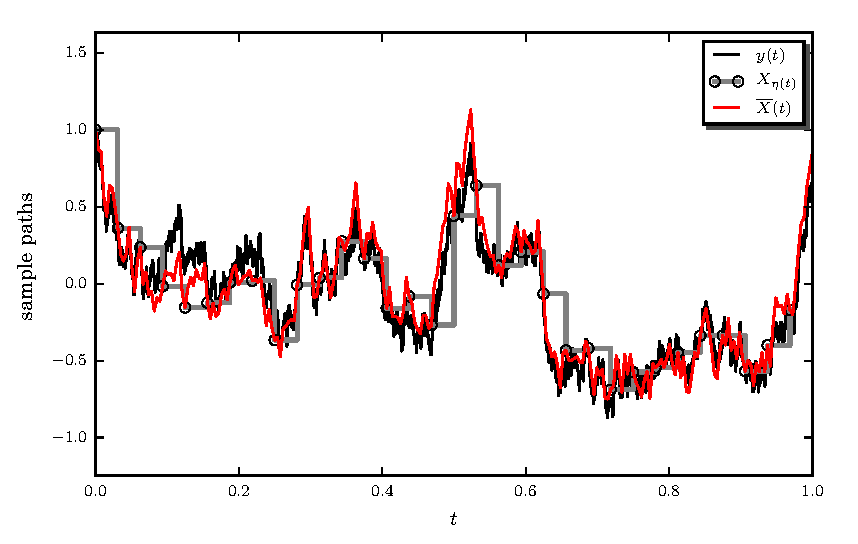
\includegraphics{papers/paperB/sections/ContinuousExtPy/ContinuousExtension.eps}
	\caption{
		The red line represents the continuous extension of the EM scheme. The continuous gray line is the 
		$Y_{\eta(t)}$ 
		process defined in \eqref{eqn:EulerMaruyama} and black line denotes the exact solution of 
		SDE \eqref{eqn:SDE}.
	}
	\label{fig:ContinuousExtension}
\end{figure}
Using the continuous extension \eqref{eqn:EMContinuousExtension}
and the uniform mean square norm, the authors use a stronger version of the ms-error%, which is given by 
$$
	\EX{\sup_{0\leq t \leq t}|y(t)-\overline{Y}(t)|^2}.
$$
%
In  order to prove strong convergence of the EM method, the following assumptions are required.
\begin{assumption}\label{ass:HighamAssumption}
	For each $R>0$ there is a positive constant $C_R$, depending only on $R$, such that
	\begin{equation}\label{ass:LipschitzCondition}
		|f(x)-f(y)|^2 \vee |g(x)-g(y)|^2 \leq C_R|x-y|^2,
		\quad
		\forall x,y\in \R^d 
		\text{ with } |x|\vee |y|\leq R.
	\end{equation}
	And for some $p>2$, there is a constant $A$ such that
	\begin{equation}
		\EX{\sup_{0\leq t\leq T}|\overline{Y}(t)|^p}
		\vee
		\EX{\sup_{0\leq t\leq T}|y(t)|^p} \leq A.
	\end{equation}
\end{assumption}
In \cite{Higham2002b}, the authors prove that the \Cref{ass:HighamAssumption} is sufficient to ensure strong 
convergence for the EM scheme, namely: 
\begin{thm}[
	{\cite[Thm 2.2]{Higham2002b}}
	]\label{thm:HighamMaoStuart}
	Under \Cref{ass:HighamAssumption}, the EM scheme \eqref{eqn:EulerMaruyama} with continuous extension
	\eqref{eqn:EMContinuousExtension}
	%\eqref{eqn:EMIntegralContinuousExtension} 
	satisfies
	\begin{equation}
		\lim_{h\to 0}
		\EX{\sup_{0\leq t\leq T}|\overline{Y}(t)-y(t)|^2}=0.
	\end{equation}
\end{thm}
	
	Applying this result, the strong convergence of an implicit split-step variant of the EM, the
SSEM method is proved . 
Their technique consist in proving each assertion of the following steps.
\begin{enumerate}[\bf{Step} 1:]
	\item
		\label{stp:EMCorrespondence}
		The SSEM for SDE \eqref{eqn:SDE1} is equivalent to the EM for the following conveniently SDE
		\begin{equation}\label{eqn:PerturbedHighamSDE}
			dy_h(t)= f_h(y_h(t))dt +g_h(y_h(t))dW(t).
		\end{equation}
	\item\label{stp:PerturbedSolution}
			The solution of the modified SDE \eqref{eqn:PerturbedHighamSDE} has bounded moments and it is 
			"close" to  $y$ the sense of the uniform mean square norm 
			$
				\EX{\sup_{0\leq t\leq T}|\cdot|^2}
			$.
	\item
	\label{stp:MethodBoundedMoments}
		Show that the SSEM method for the SDE \eqref{eqn:SDE1} has bounded moments.
	\item
		There is a continuous extension of the SSEM, $\overline{Z}(t)$, with bounded moments.
	\item
		Use the above steps and \Cref{thm:HighamMaoStuart} to conclude that
		\begin{equation}
			\lim_{h\to 0}
			\left\{
				\EX{\sup_{0\leq t\leq T}|y_h(t)-y(t)|^2}
			+
			\EX{\sup_{0\leq t\leq T}|\overline{Z}(t) -y_h(t)|^2}
			\right\}=0.
		\end{equation}
\end{enumerate}
In Chapter 4, we will use this technique.